\documentclass[runningheads]{llncs}
\usepackage{xcolor}
\usepackage{url}
\usepackage{graphicx} 
\usepackage{amssymb}
\usepackage{amsmath}
\usepackage{tikz}
\usepackage{subcaption}
\usetikzlibrary{arrows.meta, positioning, fit}

\definecolor{uf_blue}{RGB}{17,27, 150}
\definecolor{uf_orange}{RGB}{150,100,17}

\begin{document}

\title{Learning to Dispatch: A Reinforcement Learning Framework for Train Dispatch Networks}
\titlerunning{\textcolor{uf_blue}{Learning to Dispatch}}

\author{\textcolor{uf_blue}{Andres Espinosa}}
\institute{
    \textcolor{uf_orange}{Industrial and Systems Engineering \\
    University of Florida}\\
    \textcolor{uf_orange}{\email{andresespinosa@ufl.edu}}
}
\maketitle


\begin{abstract}

\end{abstract}



\section{Introduction}
\label{sse:introduction}

% What is the problem?
The Train Dispatching Problem (TDP) concerns the real-time management of train movements across a rail network, ensuring safe and efficient use of infrastructure. 
This involves deciding when and where trains should move, stop, or wait, based on factors such as schedules, track availability, and priority rules. 
Dispatching decisions must be made continuously and quickly, especially in high-traffic networks, making the problem both operationally critical and computationally challenging.

% Why does the problem exist?
Despite significant technological advances in other areas of transportation and logistics, train dispatching remains heavily reliant on human decision-makers or static rule-based systems. 
This is largely because the problem is highly combinatorial: at any given moment, there are exponentially many possible sequences of decisions that can lead to different network outcomes. 
Human dispatchers bring experience and intuition to these situations, but they are limited in how much information they can process and how consistently they can manage large-scale disruptions or optimize traffic flow over time.

% Why solve this problem?
Improving train dispatching systems has the potential to reduce passenger delays, minimize dispatching errors, and prevent network deadlocks—situations where no train can proceed without violating safety or scheduling constraints. 
Optimized dispatching can also improve energy efficiency and capacity utilization, making rail transport more competitive and sustainable. 
In dense urban transit systems or busy freight corridors, even marginal improvements in dispatching can lead to significant gains in overall network performance and reliability.

% Why solve with RL?
Reinforcement Learning (RL) offers a new approach to tackling the TDP by framing it as a sequential decision-making problem, where an agent learns to make dispatching decisions through interactions with a simulated environment. 
RL is particularly well-suited for problems with delayed consequences, dynamic environments, and large state spaces—all of which characterize train dispatching. 
With recent successes in games, robotics, and supply chain optimization, RL is emerging as a promising tool for learning policies that outperform hand-crafted heuristics in complex, real-world systems.

% Project scope.
This paper focuses on the formulation of the Train Dispatching Problem for RL-based approaches, rather than on developing a fully trained solution. 
We emphasize how the problem can be encoded as an RL task using graph structures to represent rail networks, define meaningful states, actions, and rewards, and manage constraints inherent to railway systems. 
Our goal is to provide a robust and extensible framework that future researchers and practitioners can build upon when applying RL methods to train dispatching and related infrastructure scheduling problems.

% Paper Outline
To provide a thorough understanding of our approach, the remainder of this paper is organized as follows. 
In Section~\ref{sse:background}, we present the foundational background necessary for our formulation, beginning with a formal description of the Train Dispatch Problem and its mixed-integer programming (MIP) formulation, as well as the DISPLIB benchmark format (\ref{sss:train}). 
We then outline key reinforcement learning concepts, including Markov Decision Processes (\ref{sss:reinforcement_learning}) and Deep Q-Networks, highlighting their relevance to sequential decision-making in dispatching tasks. This is followed by an introduction to Graph Neural Networks (\ref{sss:gnn}), which are critical for representing the structure of railway networks. 
Section~\ref{sse:related_work} provides a review of related literature, including recent RL applications to combinatorial scheduling, graph-based approaches, and prior work on train dispatching. 
Section~\ref{sse:formulation} details our proposed formulation, introducing Train Operation Graphs (\ref{sss:train_ops}), Resource Conflict Graphs (\ref{sss:resource_conflicts}), and the definitions of our state and action spaces (\ref{sss:state_space}, \ref{sss:action_space}). 
In Section~\ref{sse:results}, we demonstrate preliminary results from our Deep Graph Q-Network agent (\ref{sss:agent}), evaluating its performance on sample instances and visualizing its learned strategies (\ref{sss:solutions}). 
Finally, Section~\ref{sse:conclusion} outlines our conclusions and discusses future directions for scaling and refining the framework (\ref{sss:future_work}, \ref{sss:conclusion}).



\section{Problem Background}
\label{sse:background}
\subsection{Train Dispatch Problem}
\label{sss:train}
% This should cover the MIP formulation and the general outline of the problem
% This should also cover the DISPLIB data format and all that.
\subsection{Deep Reinforcement Learning}
\label{sss:reinforcement_learning}
% Cover Markov Decision Processes
% As well as DQN
Deep Reinforcement Learning (DRL) is a subfield of machine learning that combines reinforcement learning (RL) with deep learning techniques to solve complex decision-making problems. 
RL focuses on training agents to make sequential decisions by interacting with an environment, receiving feedback in the form of rewards, and learning to maximize cumulative rewards over time. 
Deep learning, on the other hand, enables the representation of high-dimensional data through neural networks, making it possible to handle complex state and action spaces.

The seminal work by Mnih et al.~\cite{drl:Mnih13} introduced the Deep Q-Network (DQN), which demonstrated the ability of DRL to learn policies directly from raw pixel inputs in Atari games. 
This approach used a convolutional neural network to approximate the Q-value function, enabling the agent to make decisions in high-dimensional state spaces. 
The success of DQN highlighted the potential of combining deep learning with RL to tackle problems that were previously intractable.

Building on this foundation, Silver et al.~\cite{drl:silver2017mastering} showcased the power of DRL in mastering the game of Go, a task long considered a grand challenge in artificial intelligence. 
Their AlphaGo system employed deep neural networks to evaluate board positions and guide search strategies, achieving superhuman performance. 
Subsequently, the AlphaZero algorithm~\cite{drl:silver2017alphazero} extended this approach to generalize across multiple games, such as chess and shogi, using a self-play mechanism and a unified reinforcement learning framework.

These advancements have established DRL as a versatile and powerful tool for solving sequential decision-making problems in diverse domains, including robotics, healthcare, and transportation systems.
\subsubsection{Markov Decision Processes}
Markov Decision Processes (MDPs) provide a mathematical framework for modeling decision-making in environments where outcomes are partly random and partly under the control of a decision-maker. An MDP is defined by the tuple $(S, A, P, R, \gamma)$:

\begin{itemize}
    \item $S$: A finite set of states representing all possible configurations of the environment.
    \item $A$: A finite set of actions available to the agent.
    \item $P(s'|s, a)$: The state transition probability function, which defines the probability of transitioning to state $s'$ given the current state $s$ and action $a$.
    \item $R(s, a)$: The reward function, which specifies the immediate reward received after taking action $a$ in state $s$.
    \item $\gamma \in [0, 1]$: The discount factor, which determines the importance of future rewards relative to immediate rewards.
\end{itemize}

The goal in an MDP is to find a policy $\pi(a|s)$, which is a mapping from states to actions, that maximizes the expected cumulative reward, also known as the return:
\[
G_t = \mathbb{E} \left[ \sum_{k=0}^\infty \gamma^k R(s_{t+k}, a_{t+k}) \right].
\]

MDPs are widely used in reinforcement learning to model environments where agents learn optimal policies through interaction and feedback.


\begin{figure}
    \centering
    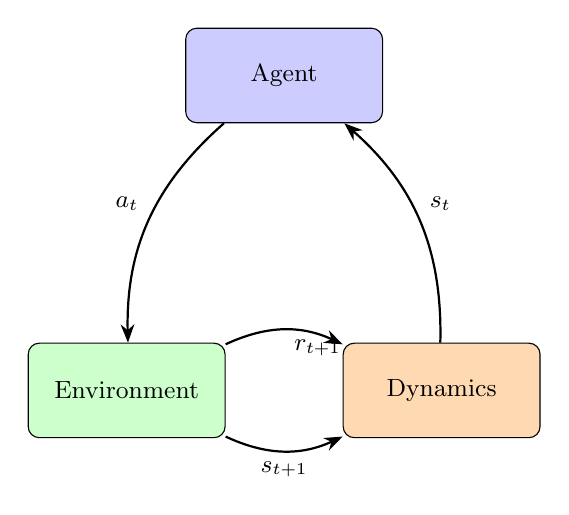
\begin{tikzpicture}[
      agent/.style={draw, rounded corners, fill=blue!20, minimum width=2.5cm, minimum height=1.2cm},
      env/.style={draw, rounded corners, fill=green!20, minimum width=2.5cm, minimum height=1.2cm},
      reward/.style={draw, rounded corners, fill=orange!30, minimum width=2.5cm, minimum height=1.2cm},
      arrow/.style={->, thick, >=Stealth},
      every node/.style={font=\small}
      ]
    
    % Nodes
    \node[agent] (agent) at (0, 2) {Agent};
    \node[env] (env) at (-2, -2) {Environment};
    \node[reward] (reward) at (2, -2) {Dynamics};
    
    % Arrows
    \draw[arrow] (agent) to[bend right=25] node[above left] {$a_t$} (env);
    \draw[arrow] (env) to[bend right=25] node[below] {$s_{t+1}$} (reward);
    \draw[arrow] (reward) to[bend right=25] node[above right] {$s_t$} (agent);
    \draw[arrow] (env) to[bend left=25] node[below right] {$r_{t+1}$} (reward);
    
    \end{tikzpicture}
    \caption{The simplified markov decision process and reinforcement learning framework.}
    \label{fig:rl_framework}
\end{figure}

\subsubsection{Deep Q-Network}
Deep Q-Networks (DQN) are a class of reinforcement learning algorithms that approximate the Q-value function using deep neural networks. The Q-value function, $Q(s, a)$, represents the expected cumulative reward of taking action $a$ in state $s$ and following the optimal policy thereafter. The DQN agent learns this function through experience replay and iterative updates.

The key components of a DQN agent are:

\begin{itemize}
    \item \textbf{Q-Network:} A neural network that takes the current state $s_t$ as input and outputs Q-values for all possible actions. The network is parameterized by weights $\theta$, which are updated during training.
    \item \textbf{Target Network:} A separate network with weights $\theta^-$, used to stabilize training by providing target Q-values. The target network is periodically updated to match the Q-network.
    \item \textbf{Experience Replay:} A buffer that stores past experiences $(s_t, a_t, r_t, s_{t+1})$. During training, mini-batches of experiences are sampled randomly from the buffer to break correlations and improve learning stability.
    \item \textbf{Bellman Equation:} The Q-network is trained to minimize the temporal difference (TD) error, defined as:
    \[
    \delta = \left[ r_t + \gamma \max_{a'} Q(s_{t+1}, a'; \theta^-) - Q(s_t, a_t; \theta) \right],
    \]
    where $\gamma$ is the discount factor.
    \item \textbf{Exploration-Exploitation Tradeoff:} The agent balances exploration (choosing random actions) and exploitation (choosing actions with the highest Q-value) using an $\epsilon$-greedy policy.
\end{itemize}

The training process involves iteratively updating the Q-network's weights $\theta$ using gradient descent to minimize the TD error. The learned Q-values guide the agent in selecting actions that maximize long-term rewards.


\begin{figure}
    \centering
    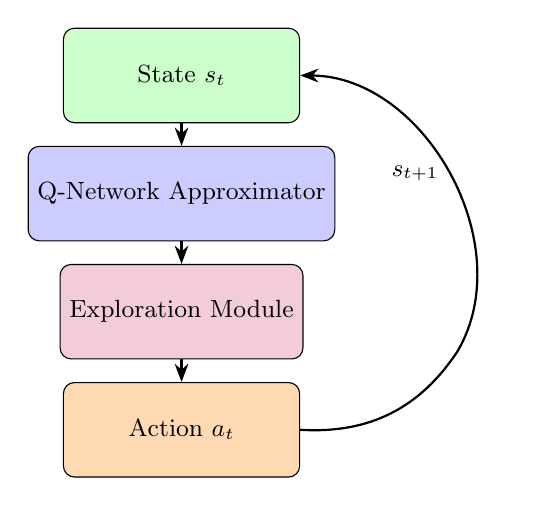
\begin{tikzpicture}[
      qnet/.style={draw, rounded corners, fill=blue!20, minimum width=3cm, minimum height=1.2cm},
      module/.style={draw, rounded corners, fill=purple!20, minimum width=3cm, minimum height=1.2cm},
      action/.style={draw, rounded corners, fill=orange!30, minimum width=3cm, minimum height=1.2cm},
      state/.style={draw, rounded corners, fill=green!20, minimum width=3cm, minimum height=1.2cm},
      arrow/.style={->, thick, >=Stealth},
      every node/.style={font=\small}
    ]
    
    % Nodes
    \node[state] (state) at (0, 2) {State $s_t$};
    \node[qnet] (qnet) at (0, 0.5) {Q-Network Approximator};
    \node[module] (explore) at (0, -1) {Exploration Module};
    \node[action] (action) at (0, -2.5) {Action $a_t$};
    
    % Arrows
    \draw[arrow] (state) -- (qnet);
    \draw[arrow] (qnet) -- (explore);
    \draw[arrow] (explore) -- (action);
    \draw[arrow] (action.east) to[bend right=30] node[right] {} ++(2,1) 
        to[bend right=60] node[left] {$s_{t+1}$} (state.east);

    \end{tikzpicture}
    \caption{Simplified Deep Q-Network action selection and feedback loop.}
    \label{fig:dqn_loop}
\end{figure}



\subsection{Graph Neural Networks}
\label{sss:gnn}
% Cover graph neural networks
Graph Neural Networks (GNNs) are a class of neural networks designed to operate on graph-structured data, where entities are represented as nodes and their relationships as edges. GNNs leverage the graph topology and node features to learn meaningful representations for tasks such as node classification, link prediction, and graph classification.

\subsubsection{Overview of GNNs}
GNNs extend traditional neural networks by incorporating message-passing mechanisms, where nodes aggregate information from their neighbors iteratively. This process enables the network to capture both local and global graph structures. The key components of GNNs include:

\begin{itemize}
    \item \textbf{Message Passing:} Nodes exchange information with their neighbors through a series of message-passing steps. At each step, a node updates its representation by aggregating messages from its neighbors.
    \item \textbf{Aggregation Functions:} Common aggregation functions include summation, mean, and max-pooling, which ensure permutation invariance in the graph structure.
    \item \textbf{Update Functions:} After aggregation, node representations are updated using learnable functions, often implemented as neural networks.
    \item \textbf{Pooling Layers:} For graph-level tasks, pooling layers summarize the entire graph into a fixed-size representation.
\end{itemize}

\subsubsection{Applications in Reinforcement Learning}
GNNs have shown significant promise in reinforcement learning (RL) for tasks involving graph-structured environments. Munikoti et al.~\cite{gnndrl:munikoti2022challengesopportunitiesdeepreinforcement} provide a comprehensive review of how GNNs enhance RL by enabling agents to reason over relational data, such as traffic networks or social graphs. They highlight the ability of GNNs to generalize across varying graph sizes and structures.

In multi-objective optimization problems, such as influence maximization in social networks, GNNs combined with meta-reinforcement learning have demonstrated effectiveness. For instance, the GraMeR framework~\cite{gnndrl:munikoti2022gramergraphmetareinforcement} leverages GNNs to learn transferable policies across different graph instances, optimizing multiple objectives simultaneously.

Devailly et al.~\cite{gnndrl:Devailly_2022} introduce IG-RL, an inductive graph reinforcement learning approach for large-scale traffic signal control. By using GNNs, their method efficiently handles massive traffic networks, enabling scalable and adaptive control strategies.

In summary, GNNs provide a powerful framework for learning on graph-structured data, with significant implications for reinforcement learning in domains like transportation, social networks, and beyond.

\section{Formulation}
\label{sse:formulation}

\subsection{Train Operation Graphs}
\label{sss:train_ops}

The Train Operation Directed Acyclic Graph (DAG) format provides a structured representation of train operations and their constraints. Conceptually, each train is modeled as a DAG, called the operations graph, with the following key components:

\begin{itemize}
    \item \textbf{Nodes:} Represent operations, each with:
    \begin{itemize}
        \item A \textbf{minimum duration} $\delta$, specifying the shortest allowable time for the operation.
        \item \textbf{Start time bounds} $[t_{\text{min}}, t_{\text{max}}]$, defining when the operation may begin.
        \item A set of \textbf{resources} required exclusively during the operation, each with an optional \textbf{release time}.
    \end{itemize}
    \item \textbf{Edges:} Define precedence constraints between operations, ensuring that dependent operations are executed in the correct order.
    \item \textbf{Entry and Exit Nodes:} The graph has a single \textbf{entry operation} (no incoming edges) and a single \textbf{exit operation} (no outgoing edges).
\end{itemize}

\subsubsection{Resources and Constraints}
Resources represent entities (e.g., track sections) that cannot be shared between trains simultaneously. Operations requiring the same resource must satisfy the following:
\begin{itemize}
    \item The \textbf{end event} of one operation must precede the \textbf{start event} of the next.
    \item The \textbf{release time} of the resource must be respected.
\end{itemize}

\subsubsection{Feasibility Conditions}
A solution is feasible if:
\begin{enumerate}
    \item Events are ordered chronologically.
    \item Each train's operations form a valid path from the entry to the exit operation.
    \item Start times respect the bounds $[t_{\text{min}}, t_{\text{max}}]$.
    \item Operation durations meet or exceed the minimum $\delta$.
    \item Resource constraints are satisfied across all trains.
\end{enumerate}

\subsubsection{Objective Function}
The objective minimizes the cost of delays, defined as:
\[
v_i = c \cdot \max(0, t - t_{\text{threshold}}) + d \cdot H(t - t_{\text{threshold}})
\]
where $c$ and $d$ are constants, $t$ is the operation's start time, and $H$ is the Heaviside step function.

\begin{figure}
    \centering
    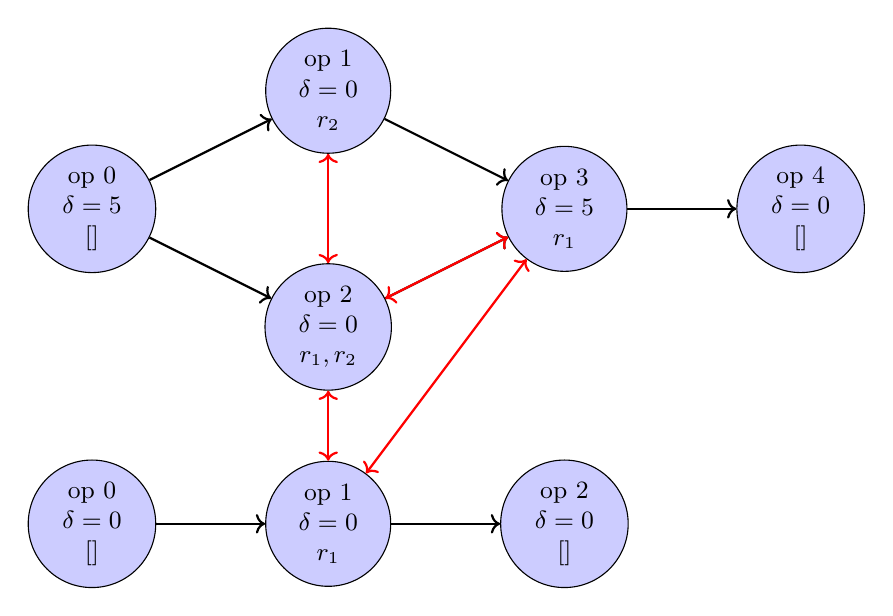
\begin{tikzpicture}[
        node/.style={circle, draw, fill=blue!20, minimum size=1.2cm, align=center},
        edge/.style={->, thick},
        resource/.style={draw, rounded corners, fill=orange!30, minimum width=1.5cm, minimum height=1cm},
        every node/.style={font=\small}
    ]
        % Nodes
        \node[node] (op0) at (0, 0) {op 0 \\ $\delta = 5$ \\ $[]$};
        \node[node] (op1) at (3, 1.5) {op 1 \\ $\delta = 0$ \\ $r_2$};
        \node[node] (op2) at (3, -1.5) {op 2 \\ $\delta = 0$ \\ $r_1, r_2$};
        \node[node] (op3) at (6, 0) {op 3 \\ $\delta = 5$ \\ $r_1$};
        \node[node] (op4) at (9, 0) {op 4 \\ $\delta = 0$ \\ $[]$};

        % Edges
        \draw[edge] (op0) -- (op1);
        \draw[edge] (op0) -- (op2);
        \draw[edge] (op1) -- (op3);
        \draw[edge] (op2) -- (op3);
        \draw[edge] (op3) -- (op4);

        % Additional DAG
        \node[node] (op0_new) at (0, -4) {op 0 \\ $\delta = 0$ \\ $[]$};
        \node[node] (op1_new) at (3, -4) {op 1 \\ $\delta = 0$ \\ $r_1$};
        \node[node] (op2_new) at (6, -4) {op 2 \\ $\delta = 0$ \\ $[]$};

        % Edges
        \draw[edge] (op0_new) -- (op1_new);
        \draw[edge] (op1_new) -- (op2_new);

        \draw[<->, red, thick] (op1) -- (op2);
        \draw[<->, red, thick] (op3) -- (op2);
        \draw[<->, red, thick] (op1_new) -- (op2);
        \draw[<->, red, thick] (op1_new) -- (op3);

    \end{tikzpicture}
    \caption{Example Train Operation DAG with resource and duration constraints.}
    \label{fig:train_dag}
\end{figure}


\subsection{Resource Conflict Graphs}
\label{sss:resource_conflicts}


\subsection{State Space}
\label{sss:state_space}

In this formulation, the state space is represented as a Directed Acyclic Graph (DAG) composed of unconnected operation graphs. 
Each node in the graph corresponds to an operation and is characterized by a feature vector that captures relevant attributes of the operation. 
The node feature vector includes the following parameters:

\begin{itemize}
    \item $x_1$: Train ID of the operation.
    \item $x_2$: Operation ID of the operation.
    \item $x_3$: Start lower bound of the operation (0 if not present).
    \item $x_4$: Start upper bound of the operation ($10^6$ if not present).
    \item $x_5$: Minimum duration of the operation (0 if not present).
    \item $x_6$: Can pick (1 if the operation has not been picked and can be picked, 0 otherwise).
    \item $x_7$: Currently picked (1 if a train has selected this operation and no successors exist, 0 otherwise).
    \item $x_8$: Picked (1 if the operation has already been picked, 0 otherwise).
    \item $x_9$: Not picked yet (1 if the operation has not been picked but can be picked in the future, 0 otherwise).
    \item $x_{10}$: Feasible (1 if the operation can be picked, 0 otherwise).
    \item $x_{11}$: Cannot be picked (1 if the operation has not been picked and cannot be picked in the future, 0 otherwise).
    \item $x_{12}$: Threshold of the operation (0 if not present).
    \item $x_{13}$: Haversine component of the operation (0 if not present).
    \item $x_{14}$: Linear delay of the operation (0 if not present).
    \item $x_{15}$: Operation start time (0 if not started yet).
    \item $x_{16}$: Operation end time (0 if not started yet).
\end{itemize}

Edges in the graph are assigned a feature vector that captures the type of relationship and resource constraints. 
The edge feature vector is defined as:
\begin{itemize}
    \item $e_1$: Operation type (1 if this edge is between two train operations, 0 o/w)
    \item $e_2$: Resource type (1 if this edge represents a resource share, 0 o/w)
    \item $e_3$: Release time (the release time of the incoming operation's resource, 0 if there is no release time or if it is an operation type edge)
\end{itemize}

This representation provides a simple yet comprehensive structure for encoding the operations and their relationships, which can be processed by a Graph Neural Network (GNN) to generate a graph embedding for downstream decision-making tasks.

\subsection{Action Space}
\label{sss:action_space}
The action space in this formulation consists of three primary actions that the agent can take at each decision step:

\begin{itemize}
    \item \textbf{Add Node:} The agent selects a specific operation node from the graph to be added to the current schedule. This action is only valid if the selected node satisfies all feasibility conditions, such as respecting precedence constraints and resource availability. The agent must choose one node from the set of feasible nodes.

    \item \textbf{Discard Node:} The agent chooses to discard a specific operation node, indicating that the operation will not be scheduled. This action is irreversible and is typically used for operations that are deemed unnecessary or infeasible to include in the schedule.

    \item \textbf{Advance Timestep:} The agent advances the simulation to the next timestep, allowing the environment to update the state of operations and resources. This action is used when no immediate scheduling decisions can be made or when the agent determines that advancing time is the optimal strategy.
\end{itemize}

Each action is represented as a discrete choice, and the agent's policy maps the current state of the environment to one of these actions. The design of this action space ensures that the agent has the flexibility to make scheduling decisions dynamically while adhering to the constraints of the problem.

% \section{Preliminary Agent Results}
% \label{sse:results}

% \subsection{Deep Graph Q-Network Agent}
% \label{sss:agent}


% \subsection{Solutions}
% \label{sss:solutions}


\section{Conclusion and Future Work}
\label{sse:conclusion}

\subsection{Future Work}
\label{sss:future_work}
This work opens several avenues for future research and development:

\subsubsection{Improved Action Space Design}
The current action space, while functional, may not fully capture the complexities and nuances of the Train Dispatching Problem. 
Future work could explore more expressive and flexible action representations, such as hierarchical or multi-step actions, to better align with real-world dispatching scenarios. 
Additionally, incorporating domain-specific heuristics or constraints directly into the action space could improve the efficiency and feasibility of the learned policies.

\subsubsection{Graph Reinforcement Learning Algorithm Development}
The integration of Graph Neural Networks (GNNs) with reinforcement learning (RL) has shown promise in handling graph-structured data. 
However, the development of specialized graph RL algorithms tailored to the unique characteristics of train dispatching remains an open challenge. 
Future research could focus on designing algorithms that leverage the structural properties of train operation and resource conflict graphs, enabling more efficient learning and better generalization across different network configurations.

\subsubsection{Extensions to Other Applications}
While this work focuses on train dispatching, the proposed framework has the potential to be adapted to other domains involving complex scheduling and resource allocation problems. 
Examples include air traffic management, urban transit systems, and supply chain logistics. 
Extending the framework to these applications would require domain-specific modifications to the state and action spaces, as well as the underlying graph representations, but could significantly broaden the impact and utility of the approach.

\subsection{Conclusion}
\label{sss:conclusion}

This honors thesis introduces a proof-of-concept reinforcement learning framework for the Train Dispatching Problem, emphasizing the formulation and potential of graph-based representations and deep learning techniques. 
By framing the problem as a Markov Decision Process and leveraging Graph Neural Networks, this work provides a foundational approach to train dispatching that is both scalable and extensible.

As a formulation-focused study, this thesis aims to inspire future research in applying reinforcement learning to complex scheduling and resource allocation problems. 
Future efforts should prioritize refining the action space, developing tailored graph reinforcement learning algorithms, and exploring applications in other domains. 
These advancements will build upon the groundwork laid here, contributing to the broader understanding and development of intelligent transportation systems.



\section{Appendix}

\begin{figure}
    \centering
    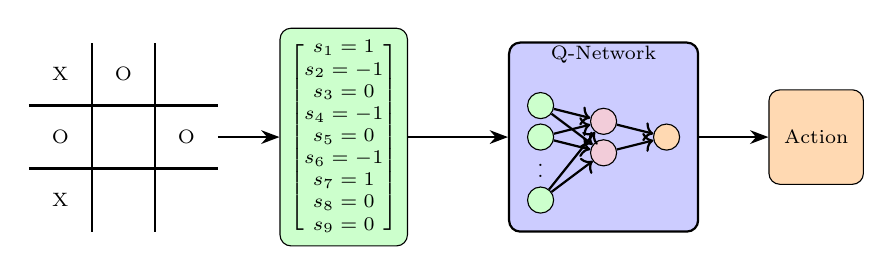
\begin{tikzpicture}[
        qnet/.style={draw, rounded corners, fill=blue!20, minimum width=1.2cm, minimum height=1.2cm},
        module/.style={draw, rounded corners, fill=purple!20, minimum width=1.2cm, minimum height=1.2cm},
        action/.style={draw, rounded corners, fill=orange!30, minimum width=1.2cm, minimum height=1.2cm},
        state/.style={draw, rounded corners, fill=green!20, minimum width=1.2cm, minimum height=1.2cm},
        arrow/.style={->, thick, >=Stealth},
        every node/.style={font=\scriptsize}
      ]
        % Vertical lines
        \draw[thick] (0.8,0) -- (0.8,2.4);
        \draw[thick] (1.6,0) -- (1.6,2.4);
        % Horizontal lines
        \draw[thick] (0,0.8) -- (2.4,0.8);
        \draw[thick] (0,1.6) -- (2.4,1.6);
        
        % Xs and Os
        \node at (0.4, 2) {X};
        \node at (1.2, 2) {O};
        \node at (2, 2) {};
        \node at (0.4, 1.2) {O};
        \node at (1.2, 1.2) {};
        \node at (2, 1.2) {O};
        \node at (0.4, 0.4) {X};
        \node at (1.2, 0.4) {};
        \node at (2, 0.4) {};

        \node[state] (state) at (4,1.2) {
            $\begin{bmatrix}
            s_1 = 1 \\ s_2 = -1 \\ s_3 = 0 \\ s_4 = -1 \\ s_5 = 0 \\ s_6 = -1 \\ s_7 = 1 \\ s_8 = 0 \\ s_9 = 0
            \end{bmatrix}$
        };
        \draw[arrow] (2.4,1.2) -- (state);

        \begin{scope}[shift={(6.5, 2)}]
            % Box and title
            \node[draw, rounded corners, thick, fill=blue!20, fit={(0, -1.6) (1.6, 0)}, inner sep=0.4cm, label={[yshift=-0.4cm]above:Q-Network}] (box) {};
            
            % Input layer
            \foreach \i in {1, 2} {
                \node[circle, draw, fill=green!20, minimum size=0.3cm] (input\i) at (0, -\i*0.4) {};
            }
            \node at (0, -1.2) {$\vdots$};
            \node[circle, draw, fill=green!20, minimum size=0.3cm] (input3) at (0, -1.6) {};
            
            % Hidden layer
            \foreach \i in {1, 2} {
                \node[circle, draw, fill=purple!20, minimum size=0.3cm] (hidden\i) at (0.8, -\i*0.4-0.2) {};
            }
            
            % Output layer
            \node[circle, draw, fill=orange!30, minimum size=0.3cm] (output) at (1.6, -0.8) {};
            
            % Connections
            \foreach \i in {1, 2, 3} {
                \foreach \j in {1, 2} {
                    \draw[->, thick] (input\i) -- (hidden\j);
                }
            }
            \foreach \i in {1, 2} {
                \draw[->, thick] (hidden\i) -- (output);
            }
        \end{scope}
        \draw[arrow] (state) -- (box);

        \node[action] (action) at (10, 1.2) {Action};

        \draw[arrow] (box) -- (action);
        
    \end{tikzpicture}
    \caption{Illustration of a Q-Network processing a Tic-Tac-Toe board state.}
    \label{fig:qnetwork_tictactoe}
\end{figure}


\begin{figure}[htbp]
    \centering

    % ANN
    \begin{subfigure}[b]{0.3\textwidth}
        \centering
        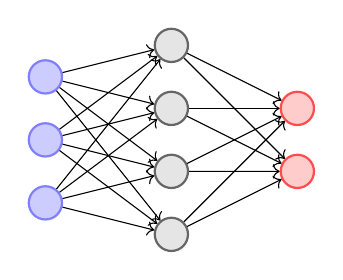
\begin{tikzpicture}[scale=0.8,
            input/.style={circle,draw=blue!50,fill=blue!20,thick,minimum size=1.2em},
            hidden/.style={circle,draw=black!60,fill=black!10,thick,minimum size=1.2em},
            output/.style={circle,draw=red!70,fill=red!20,thick,minimum size=1.2em}
        ]
            % Input Layer
            \foreach \i in {1,...,3}
                \node[input] (I\i) at (0,-\i) {};

            % Hidden Layer
            \foreach \i in {1,...,4}
                \node[hidden] (H\i) at (2,-\i+0.5) {};

            % Output Layer
            \foreach \i in {1,...,2}
                \node[output] (O\i) at (4,-\i-0.5) {};

            % Connections
            \foreach \i in {1,...,3}
                \foreach \j in {1,...,4}
                    \draw[->] (I\i) -- (H\j);

            \foreach \i in {1,...,4}
                \foreach \j in {1,...,2}
                    \draw[->] (H\i) -- (O\j);
        \end{tikzpicture}
        \caption{Fully Connected ANN}
    \end{subfigure}
    \hfill

    % CNN
    \begin{subfigure}[b]{0.3\textwidth}
        \centering
            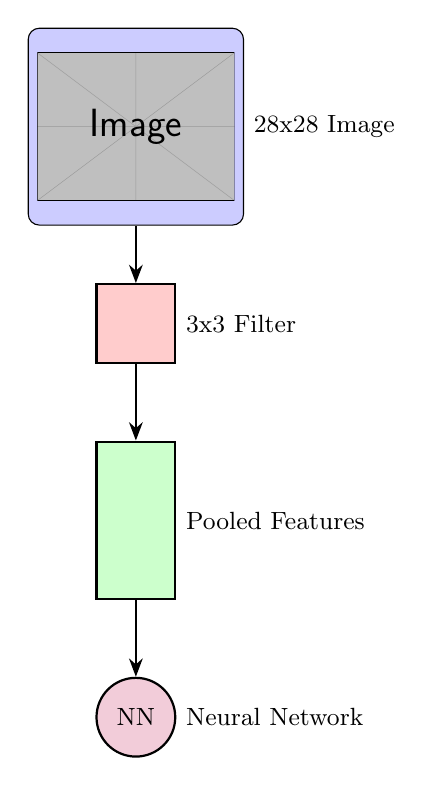
\begin{tikzpicture}[
                image/.style={draw, rounded corners, fill=blue!20, minimum width=2.5cm, minimum height=2.5cm},
                filter/.style={draw, thick, fill=red!20, minimum width=1cm, minimum height=1cm},
                feature/.style={draw, thick, fill=green!20, minimum width=1cm, minimum height=2cm},
                ann/.style={draw, thick, fill=purple!20, circle, minimum size=1cm},
                arrow/.style={->, thick, >=Stealth},
                every node/.style={font=\small}
            ]

            % Nodes
            \node[image] (input) at (0, 0) {\includegraphics[width=2.5cm]{example-image}};
            \node[filter] (filter) at (0, -2.5) {};
            \node[feature] (feature) at (0, -5) {};
            \node[ann] (ann) at (0, -7.5) {NN};

            % Labels
            \node[right] at (input.east) {28x28 Image};
            \node[right] at (filter.east) {3x3 Filter};
            \node[right] at (feature.east) {Pooled Features};
            \node[right] at (ann.east) {Neural Network};

            % Arrows
            \draw[arrow] (input) -- (filter);
            \draw[arrow] (filter) -- (feature);
            \draw[arrow] (feature) -- (ann);

            \end{tikzpicture}
            \caption{Convolutional Neural Network (CNN)}
    \end{subfigure}
    \hfill

    % GNN
    \begin{subfigure}[b]{0.3\textwidth}
        \centering
            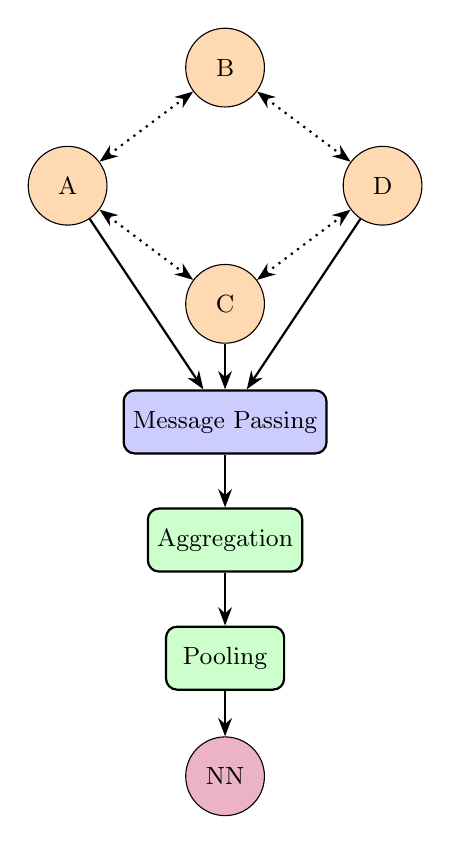
\begin{tikzpicture}[
                node/.style={circle, draw, fill=orange!30, minimum size=1cm},
                message/.style={draw, thick, fill=blue!20, minimum width=1.5cm, minimum height=0.8cm, rounded corners},
                aggregate/.style={draw, thick, fill=green!20, minimum width=1.5cm, minimum height=0.8cm, rounded corners},
                arrow/.style={->, thick, >=Stealth},
                doublearrow/.style={<->, dotted, thick, >=Stealth},
                every node/.style={font=\small}
            ]

            % Nodes
            \node[node] (A) at (0, 0) {A};
            \node[node] (B) at (2, 1.5) {B};
            \node[node] (C) at (2, -1.5) {C};
            \node[node] (D) at (4, 0) {D};

            % Edges
            \draw[doublearrow] (A) -- (B);
            \draw[doublearrow] (A) -- (C);
            \draw[doublearrow] (B) -- (D);
            \draw[doublearrow] (C) -- (D);

            % Message Passing
            \node[message] (msg) at (2, -3) {Message Passing};
            \draw[arrow] (C) -- (msg);
            \draw[arrow] (A) -- (msg);
            \draw[arrow] (D) -- (msg);

            % Aggregation
            \node[aggregate] (agg) at (2, -4.5) {Aggregation};
            \draw[arrow] (msg) -- (agg);
            % Pooling
            \node[aggregate] (pooling) at (2, -6) {Pooling};
            \draw[arrow] (agg) -- (pooling);
            

            % Output
            \node[node, fill=purple!30] (output) at (2, -7.5) {NN};
            \draw[arrow] (pooling) -- (output);
            \end{tikzpicture}
            \caption{Graph Neural Network (GNN) with Message Passing and Aggregation Steps}
    \end{subfigure}

    \caption{Simplified visual comparison of common neural network architectures}
\end{figure}

\begin{figure}
    \begin{tikzpicture}[>=Stealth, node distance=2cm and 2cm]

        % Styles
        \tikzstyle{op} = [draw, minimum width=1.8cm, minimum height=1.2cm]
        \tikzstyle{circleop} = [op, circle]
        \tikzstyle{redarrow} = [->, red, thick]
        \tikzstyle{blackarrow} = [->, thick]
        
        % Train A
        \node[op] (a0) {op 0\\$r = [\,]$};
        \node[circleop, above right=of a0] (a1) {op 1\\$r = [\,]$};
        \node[circleop, below right=of a0] (a2) {op 2\\$r = [\,]$};
        \node[circleop, right=of a1] (a3) {op 3\\$r = 1$};
        \node[op, right=of a3] (a4) {op 4\\$r = [\,]$};
        
        % Arrows for Train A
        \draw[blackarrow] (a0) -- (a1);
        \draw[blackarrow] (a0) -- (a2);
        \draw[blackarrow] (a1) -- (a3);
        \draw[blackarrow] (a3) -- (a4);
        
        % Red connections (Train A feedback or dependencies)
        \draw[redarrow] (a1) -- (a2);
        \draw[redarrow] (a2) -- (a1);
        \draw[redarrow] (a2) -- (a3);
        \draw[redarrow] (a2) -- (a2);
        
        % Train B
        \node[op, below left=4cm and 2cm of a2] (b0) {op 0\\$r = [\,]$};
        \node[circleop, right=of b0] (b1) {op 1\\$r = 1$};
        \node[op, right=of b1] (b2) {op 2\\$r = [\,]$};
        
        % Arrows for Train B
        \draw[blackarrow] (b0) -- (b1);
        \draw[blackarrow] (b1) -- (b2);
        
        % Labels
        \node[above left=0.5cm of a0] {\textbf{Train A}};
        \node[above left=0.5cm of b0] {\textbf{Train B}};
        
    \end{tikzpicture}
    
\end{figure}



\bibliographystyle{IEEEtran}
\bibliography{references}  % Assuming your .bib file is named references.bib


\end{document}



